% Chapter 6

\chapter{Derivation of PCB Layout from Schematics} % Main chapter title

\label{Chapter6} % For referencing the chapter elsewhere, use \ref{Chapter1} 

%----------------------------------------------------------------------------------------
	This section provides a detailed overview of the process and findings behind the derivation of the PCB layout from the schematic designs. This includes the PCB footprint design, the layout of the PCB, the routing of the PCB and any major challenges which were faced.\\
The PCB layout originated from early concept designs created by Paul Gardner-Stephen. This multi-layered design was used to visualise the placement of every major component within the phone. \ref{fig:Concept} displays the concept design on the top layer. 

\begin{figure}
	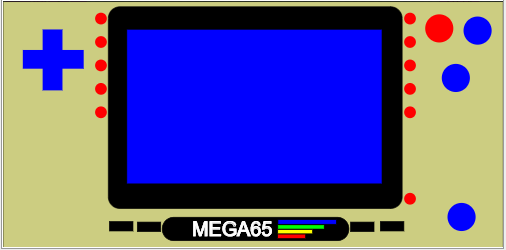
\includegraphics[width=\linewidth]{Figures/concept.png}
	\caption{Initial PCB Concept}
	\label{fig:Concept}
\end{figure}

\section{PCB Footprint Design}

	Most of the components were either downloaded from the manufacturer's approved source (eg. Digikey) or SnapEDA, components which didn't have footprints or where the footprints had incorrect dimensions were created manually using the footprint editor in Alitum. The footprints were created by following the recommended PCB outline in the desired component's datasheet. There were a few components where the datasheet was unavailable and hence the footprints were created using precise measurements of the actual item. The following list describes the footprints which were created without a datasheet, and how they were created;

\begin{itemize}
\item The footprints for the silicon moulds for the push buttons were designed in Altium using a pre-existing official footprint used for the design of the Nintendo Gameboy. This larger footprint was modified into the separate components of the DPAD buttons, the blue push buttons and the rectangular black push buttons.
\item The footprint for the modem connector was created by measuring the dimensions of the physical component. This connection part was then added to the recommended PCB layout of the modem, which was created from the datasheet. 
\end{itemize}

\section{PCB Layout}

	The start of the PCB Design process begun with a graphical editor being used to create a mockup of the MEGA65 phone. This mockup included precise measurements of the height and width of the device as well as the location of all of the major components required for the device, including the FPGA pins and the 4G Modems. THe mockup was used as the template for the PCB board with all of the measurements copied into the program. \\
	Once the schematic designs had been completed the PCB board was adjusted in Alitum to accomodate four layers. This was completed by going into Layer Stack Manager in Alitum and adding in two more signal layers. All of the schematic designs were then added into the PCB file and on top of the mockup. \ref{fig:Initial_PCB} displays one of the initial PCB layouts of the board, before the routing stage.\\

\begin{figure}
	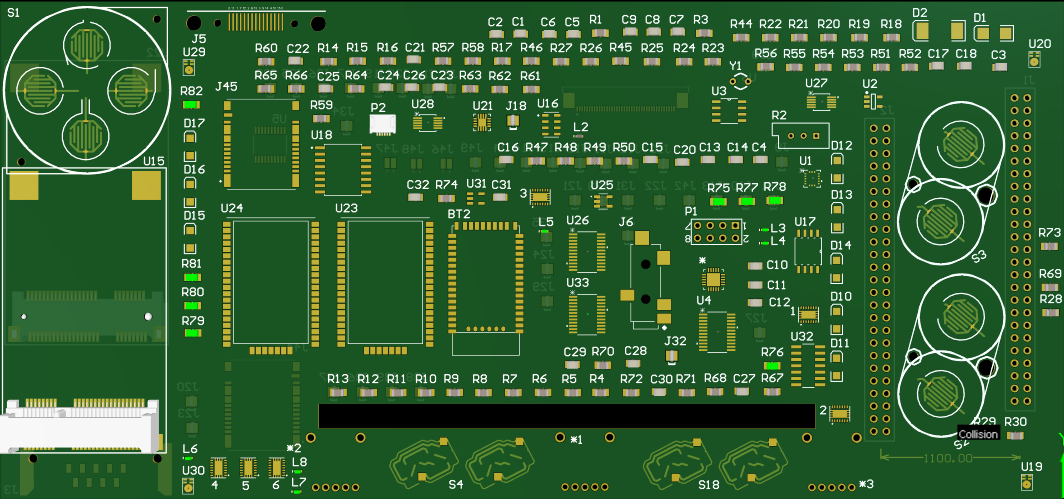
\includegraphics[width=\linewidth]{Figures/PCB.png}
	\caption{Initial PCB Layout}
	\label{fig:Initial_PCB}
\end{figure}

	It was decided near the beginning of the process that most of the ICs which would be located within the inner part of the board, would have to be positioned on the bottom layer of the board. This was needed to allow the LCD screen to lie flush with the board. It was also decided that the solder jumpers could be placed on the top side of the board below the LCD screen, as they would take up minimal height.\\

\subsection{Component Placement}
	Once all the components were placed in their relative positions they were precisely aligned into their correct positions based upon the prototype on the bench, and the concept which was made digitally. The FPGA pins were aligned first along with the connectors for both the LCD screen and the touch screen. It was essential that the large rectangular whole at the bottom of the phone was also the right width and height from the bottom of the device so that the LCD and touch ribbons would meet the connector points on the board. \ref{fig:component_placement} shows the dimensions for the touch screen connector. 

\begin{figure}
	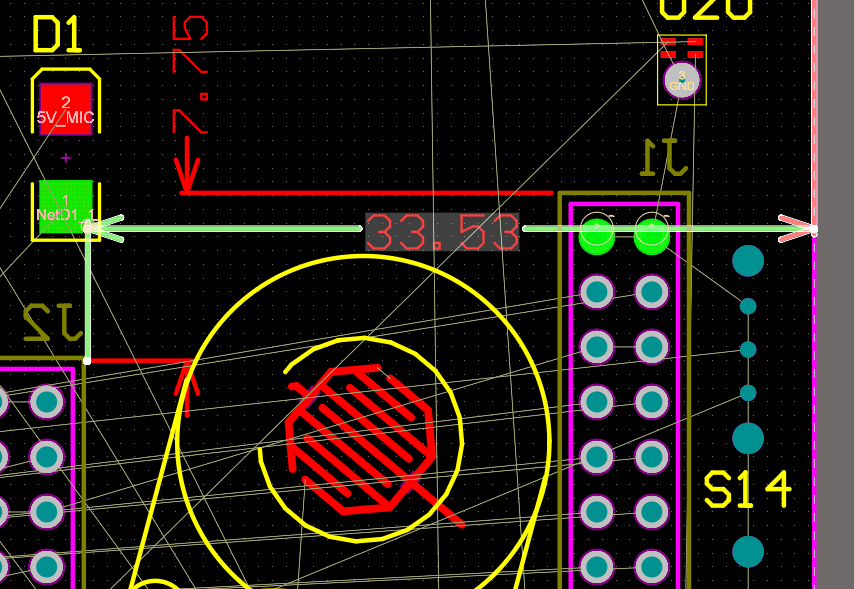
\includegraphics[width=\linewidth]{Figures/component_placement.png}
	\caption{LCD Screen Dimensioning}
	\label{fig:component_placement}
\end{figure}

\section{PCB Routing}

	Before the routing stage of the board development could begin there were a number of errors which needed to be addressed. To begin, some of the footprints weren't working correctly when imported over to the PCB file. Some of these issues were solved by going back into the schematic files and making sure that all the correct footprints were in place, for every component. Another error was that 

\section{Challenges}

	There were a number of challenges with designing the PCB board, mainly to do with the vast majority of components needed to be routed. Another challenge was discovered in the fact that the aim was to have a six-layered board, which in itselt is highly sophiscated. It was decided early on that the majority of the tricky PCB routing and design would be completed by a professional PCB designer in Germany.\\
Another challenge was found in working out the dimensions of the PCB as well as the component placement. Due to the size requirements of the board there was not a lot of room to spare with many components sitting flush with one another and required precise measurements to fit. \\
The PCB footprint design also provided a number of challenges with some of the components either not having datasheets, or their datasheets not showing the recommended PCB layout. In these cases a physical copy of the components was obtained and precisely measured before designing the component's footprint.






%----------------------------------------------------------------------------------------





